% ----------------------
  \chapter{Introducción al microprocesador CDP1802} 
% ----------------------
\label{C:antecedentes}

\section{Microprocesador CDP1802}


El microprocesador utilizado es el CDP1802 \cite{cdp1802_datasheet}, el mismo es un chip de gran escala de integración LSI (del inglés: \emph{Large Scale Integration}) de tecnología CMOS fabricado originalmente por la empresa RCA en 1974, quien también le dio el nombre COSMAC \cite{cdp1802_lab_report} (del inglés: Complementary Symmetry Monolithic Array Computer) para referirse a su arquitectura, nombre que también se utilizó para referirse a varias computadoras que fueron diseñadas durante los años en base al mismo, algunas de las cuales se mencionan en este informe. El CDP1802 fue el primer microprocesador fabricado con tecnología CMOS \cite{cdp1802_Chip_Hall_of_Fame} y posee una arquitectura y características que difieren significativamente de la mayoría de microprocesadores de 8 bits de la misma época. Además, posee un consumo de potencia ultra bajo, y no posee una velocidad de reloj mínima, permitiéndole funcionar con una señal de reloj reducida hasta \num{0}~\unit{\hertz} y luego resumir su funcionamiento sin ningún efecto negativo.

A diferencia de la mayoría de los microprocesadores, que tienen principalmente un registro de contador de programa, un registro de índice y un acumulador, el CDP1802 posee 16 registros de 16~bits de uso general, cualquiera de los cuales puede ser designado como contador de programa o registro de índice, y también posee un acumulador de 8~bits. Gran parte del set de instrucciones se encuentra dedicado a varias operaciones utilizando estos registros de uso general.

El CDP1802 también posee internamente un controlador de acceso directo de memoria o DMA (del inglés: \emph{Direct Memory Access}), permitiendo que la memoria sea leída o modificada por dispositivos externos sin necesidad de que el CDP1802 detenga la operación de su rutina principal.

Se ha optado por este microprocesador porque, a diferencia de la mayoría de los microprocesadores del mismo periodo, el CDP1802 todavía se fabrica en la actualidad, esto es debido a su estabilidad, resistencia a la radiación (como pulsos electromagnéticos), su ultra bajo consumo de energía y su habilidad para funcionar con señales de reloj de muy baja frecuencia, para disminuir el consumo de energía, cuando la velocidad de operación no es un requerimiento.

Otro aspecto del CDP1802 que lo hizo popular entre los diseñadores aeroespaciales es que estaba disponible en una versión resistente a la radiación, lo que lo hacía ideal para el duro entorno del espacio. Se utilizaron seis 1802 como cerebro de la sonda Galileo \cite{cdp1802_Nasa1}, que se lanzó en 1989 y orbitó Júpiter entre 1995 y 2003. El 1802 también ha sido utilizado en el Telescopio Espacial Hubble y además, en dispositivos comerciales como cajas registradoras, teléfonos públicos y equipamientos de audio y video.

En la figura~\ref{F:cdp1802-encapsulado} y \ref{F:cdp1802-pinout} se puede apreciar una fotografía del encapsulado del CDP1802 y la distribución de pines, respectivamente.

\begin{figure}[h!]
\centering
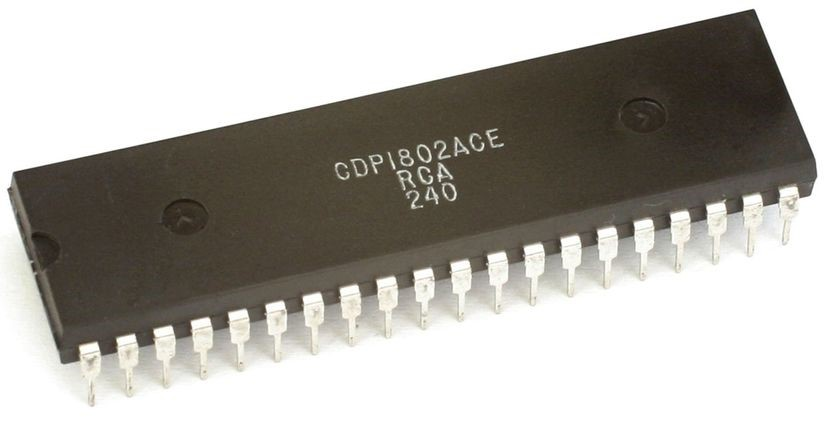
\includegraphics[width=0.5\textwidth]{./imagenes/cdp1802_encapsulado.jpg}
\caption{CDP1802 en encapsulado DIP40}
\label{F:cdp1802-encapsulado}
\end{figure}

\begin{figure}[h!]
\centering
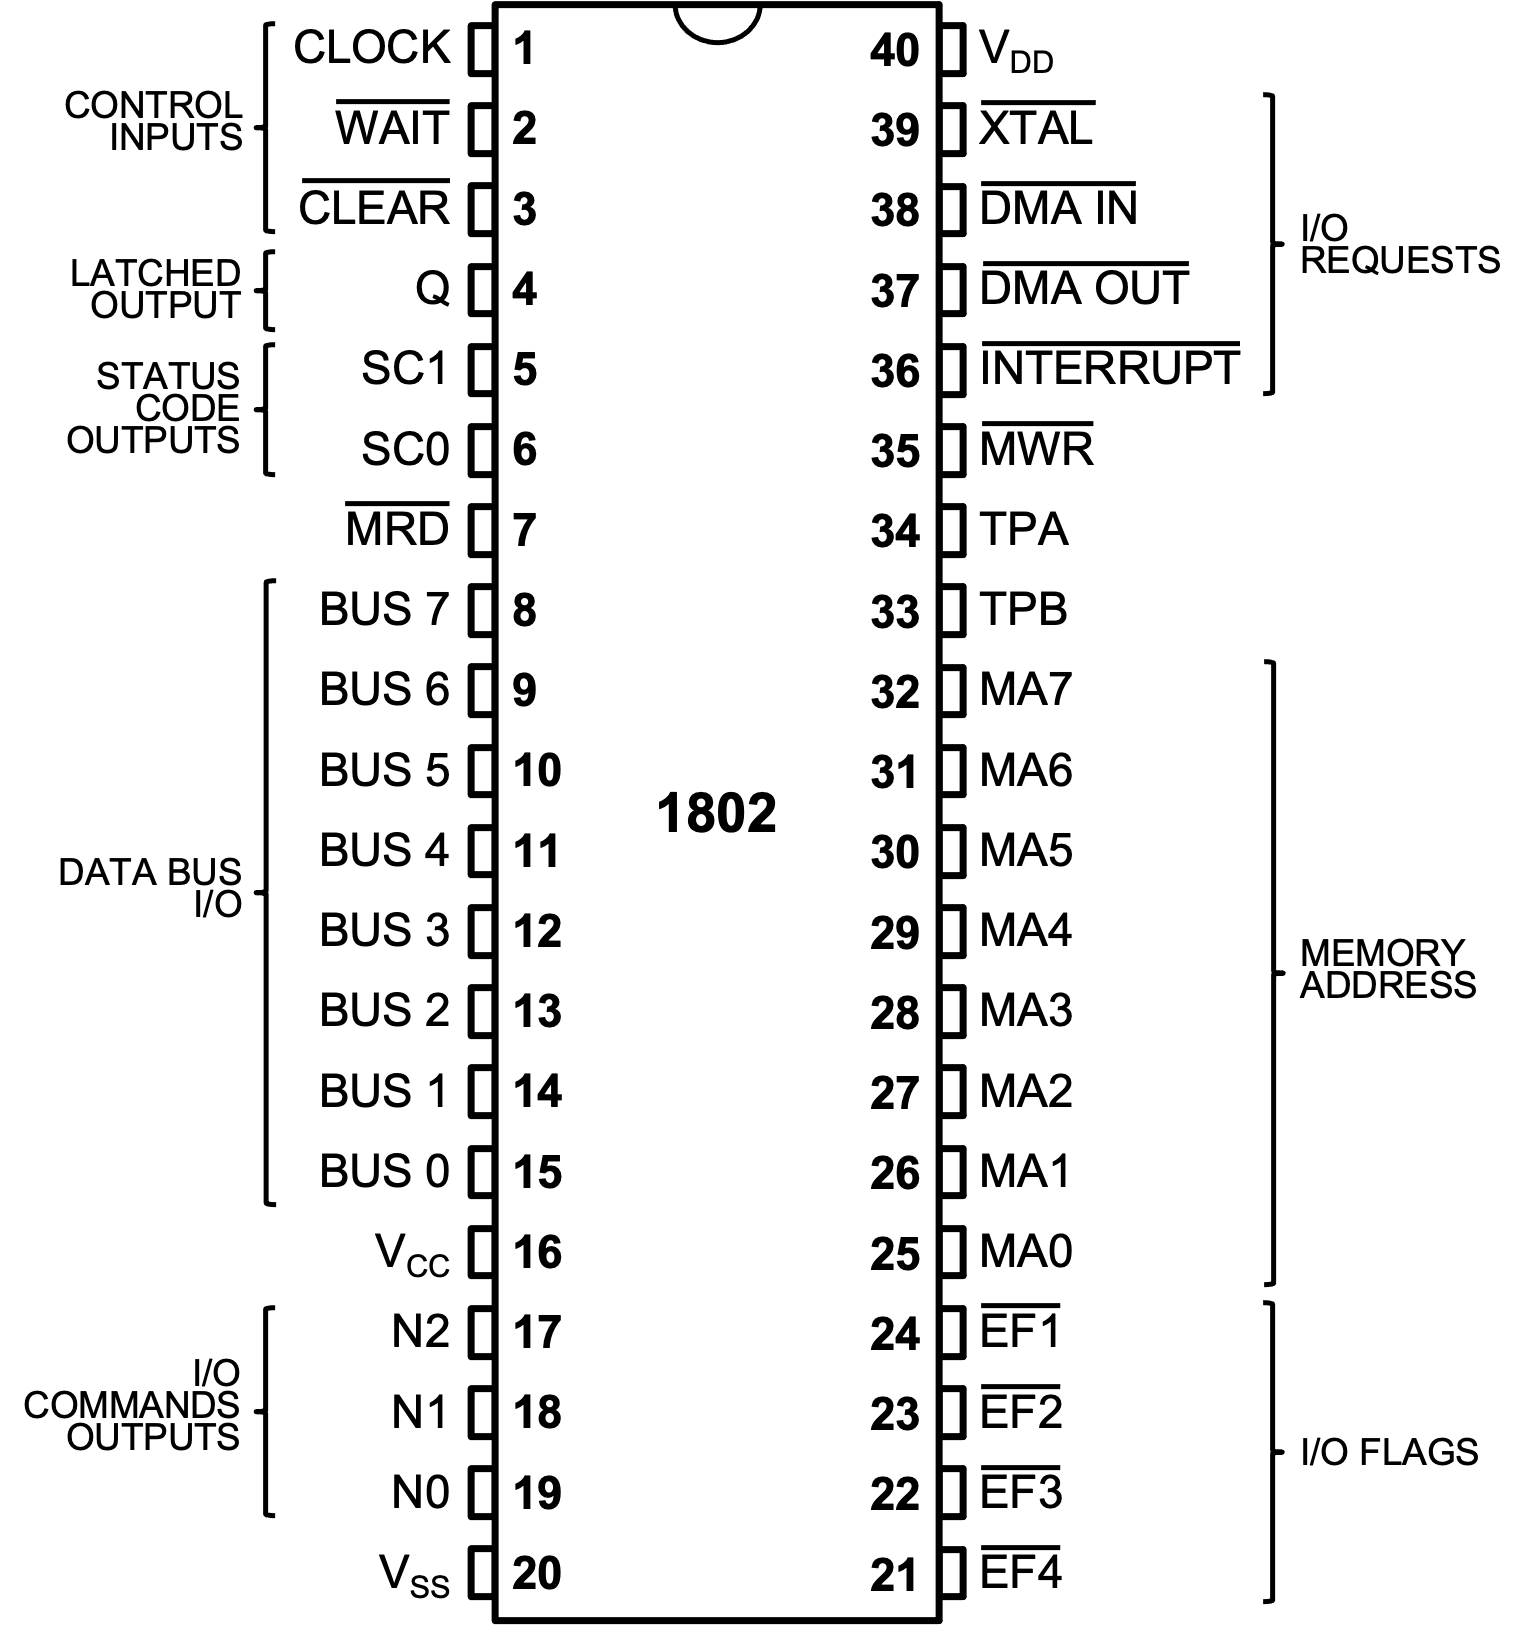
\includegraphics[width=0.65\textwidth]{./imagenes/cdp1802_pinout.png}
\caption{Distribución de pines del CDP1802}
\label{F:cdp1802-pinout}
\end{figure}

%%%%%%%%%%%%%%%%%%%%%%%%%%%%%%%%%%%%%%%%%%%%%%
\section{Computadoras basadas en el CDP1802}

\subsection{COSMAC ELF}

En la edición de agosto de 1976 de la revista Popular Electronics \cite{COSMAC_ELF_pupular_electronics}, Joseph Weisbecker detalló instrucciones para construir el COSMAC ELF basado en el CDP1802. El ELF era una computadora simplificada que permitía a los usuarios ingresar programas accionando interruptores de palanca y costaba alrededor de USD\$ 80 en partes.

\begin{figure}[h!]
\centering
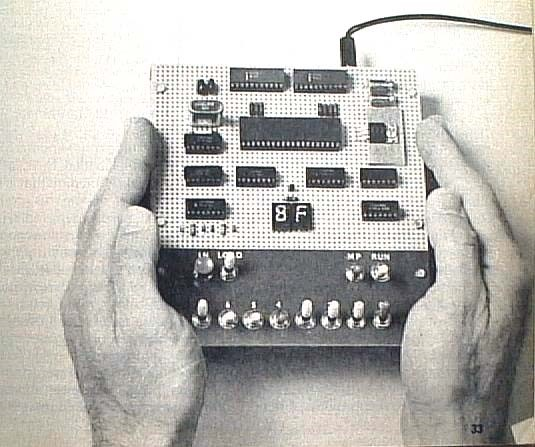
\includegraphics[width=0.7\textwidth]{./imagenes/cosmac_elf_popular_electronics.jpg}
\caption{Fotografía del COSMAC ELF de la revista Popular Electronics}
\label{F:cosmac-elf}
\end{figure}

El diseño de la computadora COSMAC ELF es simple, lo cual es así principalmente porque el CDP1802 posee un controlador DMA integrado como así también un sistema de control de dispositivos de entrada y salida, lo cual hace que no sean necesarios muchos circuitos integrados externos que de otro modo serían imprescindibles para realizar las tareas requeridas.

Una de las razones de la popularidad del CDP1802 entre los aficionados fue que su diseño facilitó la expansión de sistemas que lo utilizan y la interfaz con el mundo exterior. Los microprocesadores típicos requieren hardware de soporte y múltiples instrucciones de código máquina para utilizar periféricos de entrada y salida. Además, cuatro pines en el 1802 actúan como entradas digitales directas y con solo una instrucción de código máquina, un programa puede verificar el estado de uno de estos pines y actuar sobre el resultado. Otro pin, denominado Q, funciona como una salida de un bit que también se puede controlar con una sola instrucción de código máquina.

Una salida de un bit puede no parecer mucho, pero permite comunicación serial y el control de todo tipo de dispositivos. Tal vez lo más interesante, como señaló Weisbecker en sus artículos de Popular Electronics, es que los bucles de tiempo cuidadosamente elaborados podrían controlar con precisión la frecuencia a la que el voltaje del bit de salida cambiaba de un estado a otro, produciendo una onda cuadrada a frecuencias audibles. Esto significaba que el bit de salida podía conectarse a un altavoz y surgirían tonos musicales. Alan Turing usó una técnica similar para crear las primeras notas musicales generadas por computadora en 1951 \cite{Alan_Turing_music}.

\subsection{COSMAC ELF II}
\label{C:cosmac_elf_II}

El COSMAC ELF II es una versión mejorada de la primera COSMAC ELF, la cual incluye un teclado en lugar de interruptores para ingresar datos, además de ranuras donde pueden agregarse diferentes placas de expansión, por ejemplo, una placa de memoria RAM.

\begin{figure}[h!]
\centering
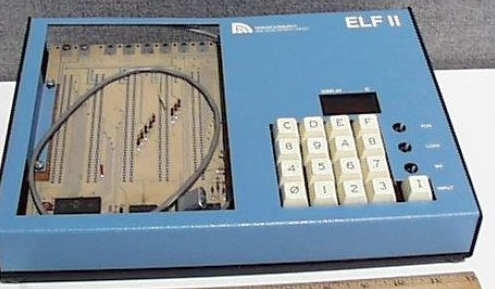
\includegraphics[width=0.7\textwidth]{./imagenes/cosmac-elf-II.png}
\caption{Fotografía obtenida en línea del COSMAC ELF II}
\label{F:cosmac-elf-II}
\end{figure}

\clearpage
\subsection{Membership Card}

La Membership Card \cite{membership-card} es una reproducción de la computadora ELF original de Popular Electronics, empaquetada para caber en una lata Altoids\textregistered~de tamaño de bolsillo. Está completamente construida con piezas y tecnología de 1980, utilizando solo componentes comunes de tecnología through hole (agujeros pasantes) y de bajo costo (sin circuitos integrados personalizados, ni componentes de montaje superficial). Para usarla no es necesario una PC moderna ni megabytes de software propietario.

\begin{figure}[ht!]
\centering
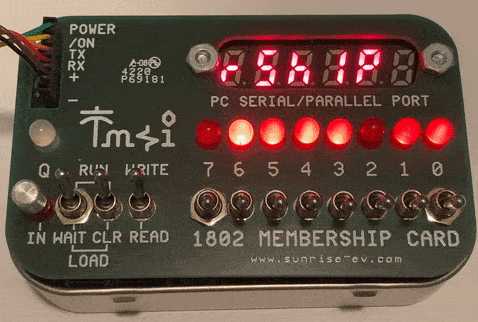
\includegraphics[width=0.6\textwidth]{./imagenes/membership-card.png}
\caption{Fotografía obtenida en línea del Membership Card}
\label{F:membership-card}
\end{figure}

La computadora está compuesta por dos placas de circuito impreso, cada una del tamaño de una tarjeta de crédito. Una es la propia Membership Card (figura~\ref{F:pcb-membership-card}), que tiene el microprocesador 1802, hasta 64k bytes de memoria, 22 bits de E/S, circuitos de reloj, reinicio, fuente de energía y además de un super-capacitor para mantener el contenido de la memoria sin energía. Se puede usar solo como un microcontrolador para proyectos como los microcontroladores Parallax BASIC Stamps o Arduino.

La segunda placa es el panel frontal (figura~\ref{F:pcb-membership-card-front-panel}). Proporciona los interruptores y los LED para un panel de control de \entreComillas{luces intermitentes}, al igual que las computadoras clásicas de antaño. Puede leer y escribir en la memoria y en los puertos de E/S manualmente, sin la ayuda de software o dispositivos externos. Los datos se muestran tanto en bits binarios individuales como en dos dígitos hexadecimales (o incluso mensajes ASCII de 6 caracteres con 4 dígitos adicionales opcionales y software apropiado).

\begin{figure}[ht!]
\centering
\subfloat[PCB Membership Card][PCB Membership Card]{
	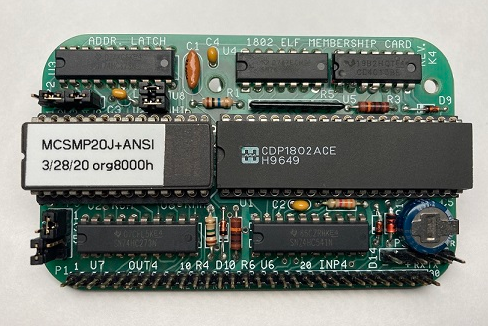
\includegraphics[width=0.6\textwidth]{./imagenes/pcb-membership-card.png}
	\label{F:pcb-membership-card}}
\\
\subfloat[PCB Membership Card Panel Frontal][PCB Membership Card Panel Frontal]{
	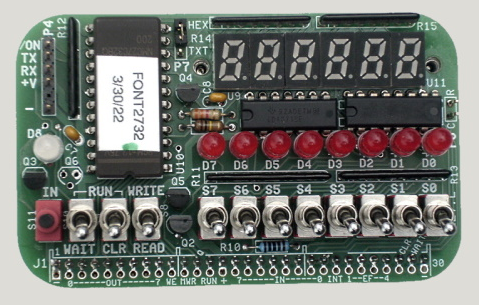
\includegraphics[width=0.6\textwidth]{./imagenes/pcb-membership-card-front-panel.png}
	\label{F:pcb-membership-card-front-panel}}
\caption{Circuitos impresos Membership Card}
\end{figure}

Un adaptador serial/USB se conecta directamente al conector de 6 pines para proporcionar alimentación y E/S serial, que permite que una terminal externa o PC cargue, guarde y ejecute programas.

\clearpage
\section{CDP1802 y la arquitectura COSMAC}

El RCA-CDP1802 es una unidad central de procesamiento (CPU) orientada a bytes que emplea la arquitectura COSMAC (Complementary Symmetry Monolithic Array Computer) y utiliza tecnología MOS (metal-oxide semiconductor) de simetría complementaria (CMOS). El microprocesador CDP1802 incluye todos los circuitos necesarios para obtener, interpretar y ejecutar instrucciones que se han almacenado en tipos estándar de memorias. También se proporcionan amplias funciones de control de entrada/salida (E/S) para facilitar el diseño del sistema.

A continuación se describen brevemente algunas características importantes del microprocesador CDP1802. La información fue obtenida del manual de usuario del mismo \cite{cdp1802_manual}.

\subsection{Características específicas}

Las funciones avanzadas y características operativas del microprocesador RCA CDP1802 incluyen:

\begin{itemize}
    \item Circuito CMOS estático, sin frecuencia de reloj mínima
    \item Rango completo de temperatura militar (-55 a +125~\unit{\degreeCelsius})
    \item Alta inmunidad al ruido y amplio rango de voltaje operativo
    \item Compatibilidad con TTL
    \item Reloj monofásico; oscilador opcional, en chip, controlado por cristal
    \item Control simple de reinicio, inicio y pausa
    \item Organización paralela de 8 bits con bus de datos bidireccional
    \item Facilidad de carga de programa incorporada
    \item Cualquier combinación de RAM y ROM estándar a través de una interfaz común
    \item Direccionamiento directo de memoria hasta 65.536 bytes
    \item Modo de E/S programable flexible
    \item Modo de interrupción del programa
    \item Recurso DMA (Direct Memory Access) en chip
    \item Cuatro entradas de bandera de E/S comprobables directamente por instrucción de salto
    \item Puertos de salida programable
    \item Formato de instrucción de uno a tres bytes con tiempo de ejecución de dos ciclos de máquina para cada instrucción\footnote{Excepto las instrucciones de saltos largos (long-branch instructions) y salteo largo (long-skip instructions) que requieren tres ciclos de máquina.}
    \item 91 instrucciones de uso simple
    \item Compatibilidad de software con el CDP1801
    \item Matriz de registros generales de 16~X~16 para usar como múltiples contadores de programa, punteros de datos o registros de datos
\end{itemize}

\subsection{Organización del sistema}

La figura~\ref{F:system_organization} ilustra un sistema informático típico que incorpora el microprocesador CDP1802. Las operaciones que se pueden realizar incluyen:

\begin{itemize}
    \item[a)] Control de dispositivos de E/S
    \item[b)] Transferencia de datos o información de control entre dispositivos de E/S y memoria
    \item[c)] Movimiento de datos entre diferentes posiciones de memoria
    \item[d)] Interpretación o modificación de bytes guardados en memoria
\end{itemize}

La memoria puede comprender cualquier combinación de RAM y ROM hasta un máximo de \num{65536}~bytes. La ROM (memoria de solo lectura) se utiliza para el almacenamiento permanente de programas, tablas y otros tipos de datos fijos. Se requiere RAM (memoria de acceso aleatorio) para los sistemas informáticos de propósito general que requieren cambios frecuentes de programa. También se requiere RAM para el almacenamiento temporal de datos variables. El tipo de memoria y la capacidad de almacenamiento requerida están determinados por la aplicación específica del sistema.

\begin{figure}[ht!]
\centering
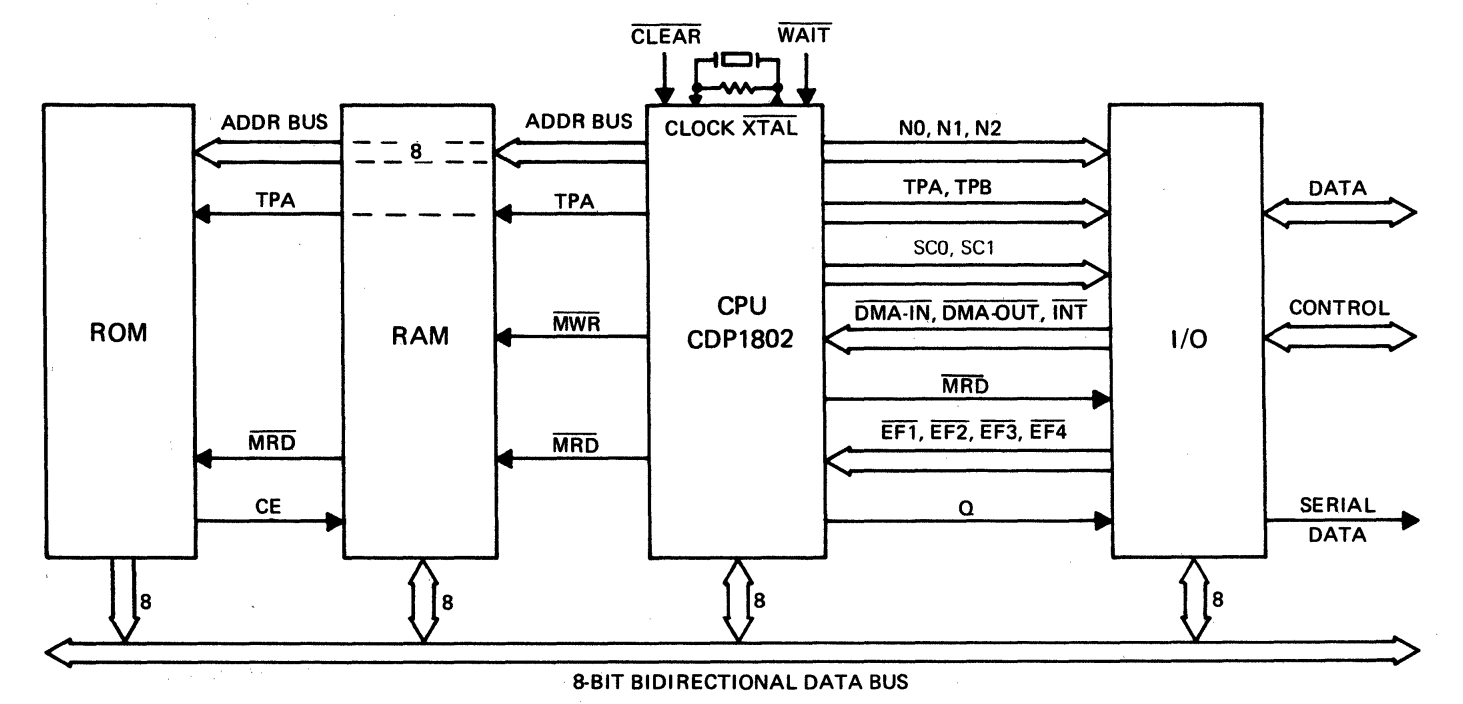
\includegraphics[width=1\textwidth]{./imagenes/system_organization.png}
\caption{\centering Diagrama de bloques de un sistema computacional típico usando el microprocesador CDP1802}
\label{F:system_organization}
\end{figure}

Los datos se transfieren desde o hacia el microprocesador entre los dispositivos de E/S y las memorias por medio de un \textbf{bus de datos bidireccional común de ocho bits} (BUS0-BUS7).

Las instrucciones de entrada/salida generan un \textbf{código N de tres bits} (N0, N1 y N2). El uso del código N para especificar un dispositivo de E/S permite un control simple y económico de una pequeña cantidad de dispositivos de E/S.

El microprocesador cuenta con \textbf{cuatro entradas que actúan como banderas de E/S} ($ \overline{\text{EF1}} $, $ \overline{\text{EF2}} $, $ \overline{\text{EF3}} $ y $ \overline{\text{EF4}} $). Los dispositivos de E/S pueden controlar estas entradas en cualquier momento para señalar al CDP1802 que se requiere una transferencia de bytes, que se ha producido una condición de error, etc. Estos indicadores también se pueden utilizar como líneas de entrada binaria si se desea. Se pueden probar mediante instrucciones CDP1802 para determinar si están activos o no.
El uso de las entradas de bandera debe coordinarse con los programas que las prueban.

También está disponible un \textbf{pin de salida} (Q), cuyo valor es controlado por instrucciones. Esta línea Q, bajo el control del programa, puede activar o señalar dispositivos de E/S. También se puede usar en conjunto con una de las entradas de bandera ($ \overline{\text{EFx}} $) para formar una interfaz de comunicación serial.

Los circuitos de E/S pueden activar una \textbf{línea de interrupción de programa} ($ \overline{\text{INT}} $) en cualquier momento para obtener una respuesta inmediata del microprocesador. La interrupción hace que el CDP1802 suspenda su secuencia de programa actual y ejecute una secuencia predeterminada de operaciones diseñadas para responder a la condición de interrupción. Después de atender la interrupción, el CDP1802 reanuda la ejecución del programa interrumpido. Se puede hacer que el CDP1802 ignore la línea de interrupción reiniciando su \textbf{flip-flop de habilitación de interrupción (IE)}.

Se proporcionan dos líneas de E/S adicionales para tipos especiales de transferencia de bytes entre la memoria y los dispositivos de E/S. Estas líneas se denominan \textbf{líneas de acceso directo a memoria} (Direct Memory Access - DMA). La activación de la línea $ \overline{\text{DMA-IN}} $ hace que un byte de entrada se almacene inmediatamente en una ubicación de memoria sin la intervención del programa que se está ejecutando. La línea $ \overline{\text{DMA-OUT}} $ hace que un byte se transfiera inmediatamente desde la memoria a los circuitos de salida solicitantes. Se utiliza un registro de puntero de memoria incorporado para indicar la ubicación de memoria para los ciclos de DMA. El programa establece inicialmente este puntero en una ubicación de memoria inicial. Cada transferencia de byte DMA incrementa automáticamente el puntero a la siguiente ubicación de memoria. La activación repetida de una línea DMA puede provocar la transferencia de cualquier número de bytes consecutivos hacia y desde la memoria, independientemente de la ejecución simultánea del programa.

Los circuitos de dispositivos de E/S pueden provocar la transferencia de datos al activar una línea de bandera ($ \overline{\text{EFx}} $), la línea de interrupción ($ \overline{\text{INT}} $) o una línea DMA ($ \overline{\text{DMA-IN}} $ o $ \overline{\text{DMA-OUT}} $). El programa debe muestrear las líneas de bandera para determinar cuándo se activan y se utilizan para detectar señales relativamente lentas. La activación de la línea de interrupción provoca una respuesta inmediata, independientemente del programa que se esté ejecutando actualmente, suspendiendo la operación de ese programa y permitiendo una respuesta en tiempo real. El uso de DMA proporciona la respuesta más rápida con la menor perturbación del programa.

Se proporciona un \textbf{código de estado de dos bits} (SC0 y SC1) y \textbf{dos líneas de temporización} (TPA y TPB) para que los utilicen los circuitos de dispositivos de E/S. Estas cuatro señales permiten la sincronización de circuitos de E/S con ciclos operativos internos del CDP1802. El código de estado indica si el CDP1802 está respondiendo a una solicitud de DMA, respondiendo a una solicitud de interrupción, obteniendo una instrucción o ejecutando una instrucción; esto se encuentra resumido en la tabla~\ref{T:state_codes}. Los sistemas de memoria y de E/S utilizan las señales de temporización para señalar un nuevo código de estado del procesador, bloquear bits de dirección de memoria (para obtener direccionamiento de hasta 16 bits con solo 8 pines de dirección), tomar datos de memoria del bus y establecer o restablecer los flip-flops del controlador de E/S.

% Please add the following required packages to your document preamble:
% \usepackage{multirow}
\begin{table}[ht!]
\caption{Códigos de estado}
\label{T:state_codes}
\begin{tabular}{|l|ll|}
\hline
\multicolumn{1}{|c|}{\multirow{2}{*}{State Type}} & \multicolumn{2}{l|}{State Code} \\ \cline{2-3} 
\multicolumn{1}{|c|}{}                            & \multicolumn{1}{l|}{SC1}  & SC0 \\ \hline
S0 (Fetch)                                        & \multicolumn{1}{l|}{L}    & L   \\ \hline
S1 (Execute)                                      & \multicolumn{1}{l|}{L}    & H   \\ \hline
S2 (DMA)                                          & \multicolumn{1}{l|}{H}    & L   \\ \hline
S3 (Interrupt)                                    & \multicolumn{1}{l|}{H}    & H   \\ \hline
\end{tabular}
\end{table}

El CDP1802 proporciona ocho líneas de dirección de memoria (MA0-MA7). Estas ocho líneas proporcionan direcciones de memoria de 16 bits en forma de dos bytes de 8 bits sucesivos. El byte de dirección más significativo (de orden superior) aparece primero en las ocho líneas de dirección, seguido del byte de dirección menos significativo (de orden inferior). El número de bits de orden superior necesarios para seleccionar una ubicación de byte de memoria única depende del tamaño de la memoria. Por ejemplo, una memoria de 4096 bytes requeriría una dirección de 12 bits. Esta dirección de 12 bits se obtiene combinando 4 bits del byte de dirección de orden superior con los 8 bits del byte de dirección de orden inferior. Uno de los dos pulsos de temporización del CDP1802 se puede usar para introducir los bits de orden superior requeridos en un latch de dirección (registro paralelo de 8 bits) cuando aparecen en las ocho líneas de dirección.

Cuatro líneas adicionales completan la interfaz del sistema del microprocesador. Una entrada de reloj monofásica (CLOCK) determina la velocidad de funcionamiento. El reloj externo se puede detener y comenzar nuevamente, continuando con la operación del CDP1802 donde se había quedado antes de detenerse el reloj. La construcción del circuito de reloj se simplifica mediante el uso de la entrada $ \overline{\text{XTAL}} $. Se conecta un cristal entre $ \overline{\text{XTAL}} $ y la entrada de reloj CLOCK, por lo cual no se necesitan componentes activos. La línea de entrada $ \overline{\text{CLEAR}} $ inicializa el microprocesador y su liberación inicia la ejecución de las instrucciones. La línea $ \overline{\text{WAIT}} $ suspende la operación de la CPU limpiamente. La activación simultánea de $ \overline{\text{CLEAR}} $ y $ \overline{\text{WAIT}} $ pone a la CPU en un modo de carga de programa. La tabla~\ref{T:CDP1802_modes} resume estos modos de operación.

\begin{table}[ht!]
\caption{Modos del CDP1802}
\label{T:CDP1802_modes}
\begin{tabular}{|l|l|l|}
\hline
      &      & \\
$ \overline{\text{CLEAR}} $ & $ \overline{\text{WAIT}} $ & MODE  \\[0.3cm] \hline
L     & L    & Load  \\
L     & H    & Reset \\
H     & L    & Pause \\
H     & H    & Run   \\ \hline
\end{tabular}
\end{table}

\subsection{Notación de la arquitectura COSMAC}

La figura~\ref{F:estructura_interna} ilustra la estructura interna del microprocesador COSMAC CDP1802. Esta arquitectura se basa en una matriz de registros que comprende dieciséis registros tipo \textbf{scratch-pad} de 16 bits de propósito general. Cada registro (denominados \textbf{R}) se designa mediante un código binario de 4 bits. Aquí se utilizará la \textbf{notación hexadecimal (hex)} para referirse a códigos binarios de 4 bits; en la tabla~\ref{T:dec_bin_hex} se encuentra el equivalente decimal y binario de todos los dígitos hexadecimales.
Siguiendo la notación hexadecimal, podemos referirnos a los registros 3 y 12 como \textbf{R(3)} y \textbf{R(C)}, respectivamente. De esta manera nos referimos a los registros de 16~bits; sin embargo, podemos referirnos a los bytes que lo componen como \textbf{R(3).0} y \textbf{R(3).1}, que indican el byte menos significativo y más significativo de \textbf{R(3)}, respectivamente.

\begin{figure}[ht!]
\centering
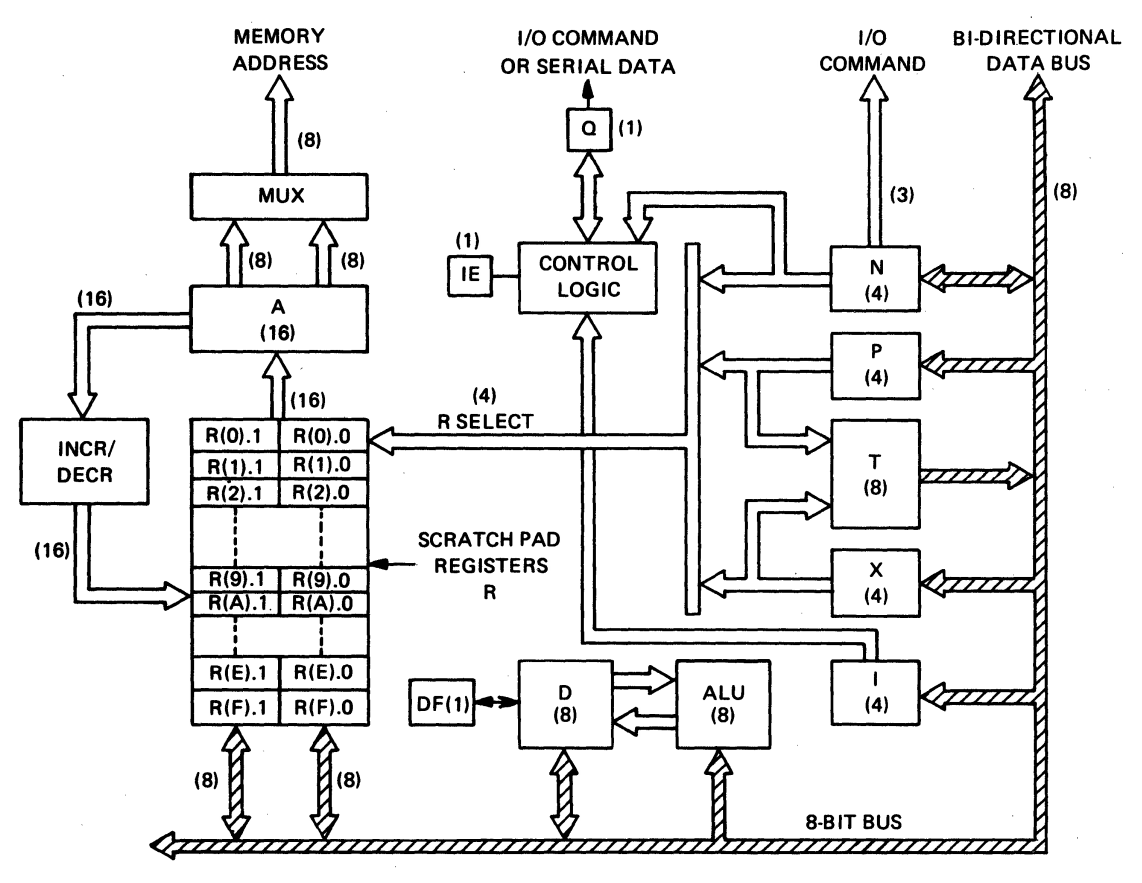
\includegraphics[width=1\textwidth]{./imagenes/estructura_interna.png}
\caption{Estructura interna del microprocesador CDP1802}
\label{F:estructura_interna}
\end{figure}

\begin{table}[ht!]
\caption{Numeración decimal, binaria y hexadecimal}
\label{T:dec_bin_hex}
\begin{tabular}{|c|c|c|}
\hline
Decimal & Binario & Hexadecimal \\ \hline \hline
0       & 0000    & 0           \\ \hline
1       & 0001    & 1           \\ \hline
2       & 0010    & 2           \\ \hline
3       & 0011    & 3           \\ \hline
4       & 0100    & 4           \\ \hline
5       & 0101    & 5           \\ \hline
6       & 0110    & 6           \\ \hline
7       & 0111    & 7           \\ \hline
8       & 1000    & 8           \\ \hline
9       & 1001    & 9           \\ \hline
10      & 1010    & A           \\ \hline
11      & 1011    & B           \\ \hline
12      & 1100    & C           \\ \hline
13      & 1101    & D           \\ \hline
14      & 1110    & E           \\ \hline
15      & 1111    & F           \\ \hline
\end{tabular}
\end{table}

Tres registros de 4 bits denominados \textbf{N}, \textbf{P} y \textbf{X} contienen los códigos binarios de 4 bits (dígitos hexadecimales) que se utilizan para seleccionar registros de 16~bits individualmente. La notación \textbf{R(X)}, \textbf{R(N)} o \textbf{R(P)} se usa para referirse a un registro de 16~bits seleccionado por el código de 4 bits en \textbf{X}, \textbf{N} o \textbf{P}, respectivamente.

De esta manera, la siguiente notación denota que la parte baja de \textbf{R(N)} es transferida al registro de 8~bits \textbf{D}, que es similar al acumulador encontrado comúnmente en microprocesadores, y el bit \textbf{DF} es el Carry de \textbf{D}, y el mismo pasa a \entreComillas{1} si el resultado de una operación desborda \textbf{D}.

\begin{equation*}
    \text{ R(N).0 } \rightarrow \text{ D }
\end{equation*}

También se puede leer directamente de la memoria utilizando uno de los registros de trabajo de 16 bits para realizar el direccionamiento para la lectura, como se muestra en la siguiente notación.

\begin{equation*}
    \text{ M(R(X)) } \rightarrow \text{ D }
\end{equation*}

El flip-flop interno \textbf{Q} se puede configurar o restablecer mediante instrucciones, y también existen instrucciones de salto condicional en base al valor de \textbf{Q}. El estado de \textbf{Q} también está disponible como salida del microprocesador.

\paragraph{Formato de instrucciones}

La operación del microprocesador se especifica mediante una secuencia de códigos de instrucción almacenados en la memoria externa. Se aplica un formato de instrucción de un byte para la mayoría de las instrucciones. Los dos dígitos hexadecimales de 4~bits que componen cada byte de instrucción se designan como \textbf{I} y \textbf{N}, como se muestra en la figura~\ref{F:instruction_format}.

\begin{figure}[ht!]
\centering
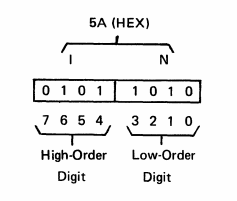
\includegraphics[width=0.35\textwidth]{./imagenes/instruction_format.png}
\caption{Formato de instrucción}
\label{F:instruction_format}
\end{figure}

Para la mayoría de las instrucciones, la ejecución requiere dos ciclos máquina. El primer ciclo (Fetch Cycle) lee el byte de instrucción apropiado de la memoria y almacena los dos dígitos de instrucción hexadecimales en los registros internos \textbf{I} y \textbf{N}. Los valores en \textbf{I} y \textbf{N} especifican la operación que se realizará durante el segundo ciclo máquina. \textbf{I} especifica el tipo de instrucción. Según la instrucción, \textbf{N} designa un registro de trabajo o, en otros casos, actúa como un código especial.

Las instrucciones normalmente se ejecutan en secuencia. Se utiliza un contador de programa para direccionar sucesivamente los bytes de memoria que representan las instrucciones. En la arquitectura COSMAC, cualquiera de los registros de trabajo general de 16~bits puede ser utilizado como contador de programa. El valor del dígito hexadecimal contenido en el registro \textbf{P} determina qué registro de trabajo se está utilizando actualmente como contador de programa. Las operaciones realizadas por el ciclo de búsqueda (Fetch Cycle) se representan de la siguiente manera.

\begin{equation*}
    \text{ M(R(P)) } \rightarrow \text{ I,N ; R(P)+1} \rightarrow \text{ R(P) }
\end{equation*}

\paragraph{Contadores de programa múltiples}

Un contador de programa es un registro que apunta a la siguiente instrucción a buscar y ejecutar. La arquitectura COSMAC brinda la capacidad única de especificar, en una sola instrucción (instrucción SEP), cualquiera de los 16 registros de trabajo como contador de programa. Esta característica hace posible mantener punteros a varios programas diferentes simultáneamente y transferir el control rápidamente de uno a otro. Un puntero a un programa que atiende una solicitud de interrupción, o la posibilidad de crear subrutinas que pueden operar sin RAM, son solo dos ejemplos de esta función.

